\renewcommand{\parttitle}{IMAGES AND COMMENTS}

\section*{Influence of strut position on divergence}
\noindent
\begin{minipage}[c]{0.54\textwidth}
\centering
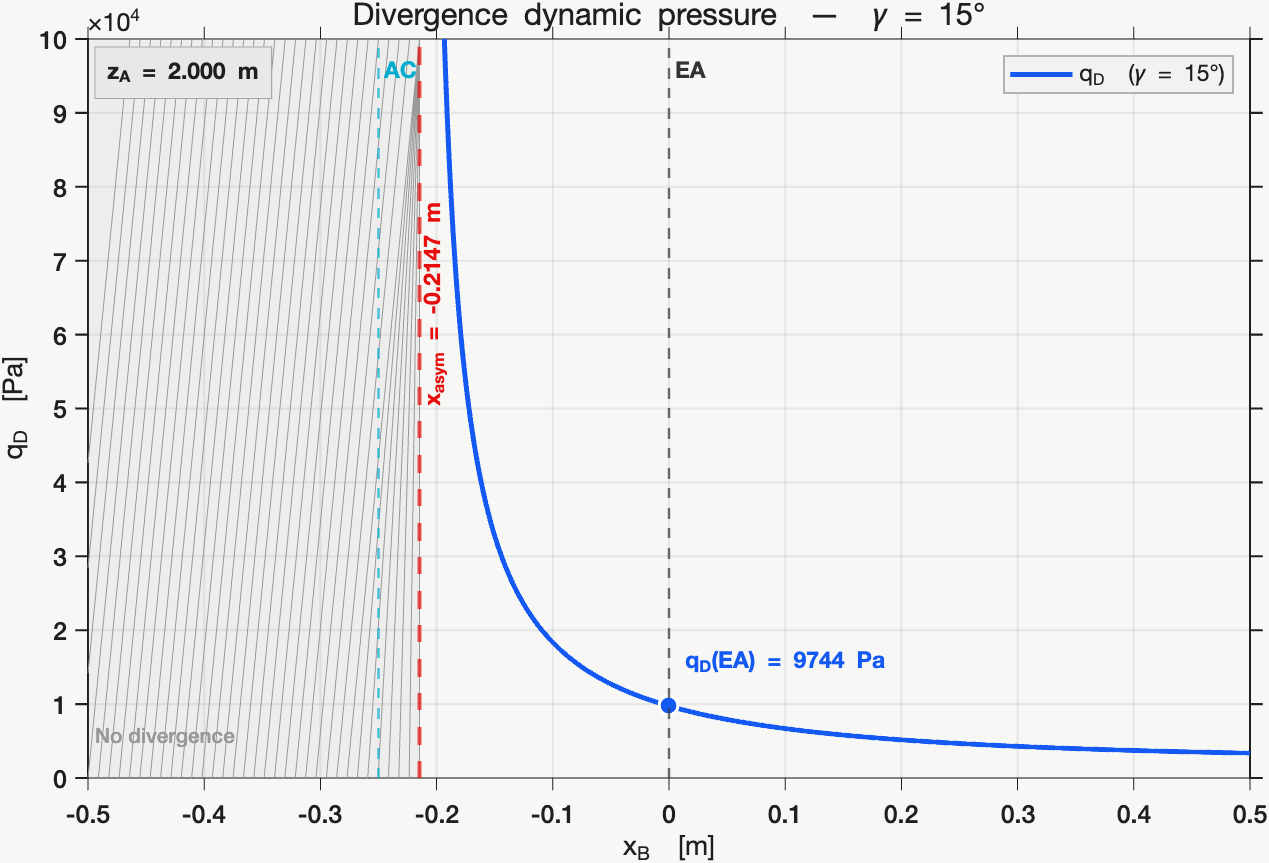
\includegraphics[width=\textwidth]{report/img/qD_vs_xB_gamma15.png}
\captionof{figure}{$q_D$ vs.\ $x_B$ for $\gamma=15^\circ$.}
\label{fig:qD_xB_gamma15}
\end{minipage}%
\hfill%
\begin{minipage}[c]{0.43\textwidth}
$q_D$ is highly sensitive to $x_B$. A vertical asymptote at $x_B\simeq-0.2147\ \mathrm{m}$ separates two regimes:
\begin{itemize}
    \item[$\bullet$] \textbf{Right:} divergence at positive $q_D$, dropping rapidly toward the elastic axis ($q_D\approx9.7\times10^3\ \mathrm{Pa}$).
    \item[$\bullet$] \textbf{Left:} flexural--torsional stabilization suppresses static divergence entirely.
\end{itemize}
\paragraph{Limitations.} No-divergence region holds within the linear model only -- flutter and control reversal remain unconstrained. Forward strut placement may incur buckling/mass penalties and is sensitive to geometric tolerances near the asymptotic boundary.
\end{minipage}


\section*{Influence of \texorpdfstring{$\gamma$}{gamma} on the control effectiveness}
\begin{figure}[htbp]
\begin{minipage}[c]{0.43\textwidth}
$x_B$ fixed; $E_C=L/L_R$ with $E_C=1$ rigid limit, $E_C>1$ amplification, $E_C<0$ reversal.
All curves start at $E_C=1$. Three regimes:
\begin{itemize}
    \item[$\bullet$] \textbf{Low $\gamma$ ($10^\circ$, $12.5^\circ$):} $E_C>1$ -- elastic twist amplifies aileron effect -- then blocked by divergence; displayed value is actually $q_D$, not $q_C$.
    \item[$\bullet$] \textbf{Intermediate ($15^\circ$):} monotonic decrease, genuine reversal at $q_C=29\,702\ \mathrm{Pa}$.
    \item[$\bullet$] \textbf{High $\gamma$ ($17.5^\circ$, $20^\circ$):} detrimental coupling from low $q$; $q_C=24\,685$ and $21\,427\ \mathrm{Pa}$ -- reversal pressure decreases with $\gamma$.
\end{itemize}
$E_C\sim[\det\mathbf{K}_{\mathrm{TOT}}]^{-1}$; negative branch past divergence is a mathematical artefact. $\gamma$ controls sign and magnitude of aeroelastic feedback: low $\gamma\to$ favorable amplification (divergence governs); high $\gamma\to$ early control reversal.
\end{minipage}
\hfill
\begin{minipage}[c]{0.54\textwidth}
\centering
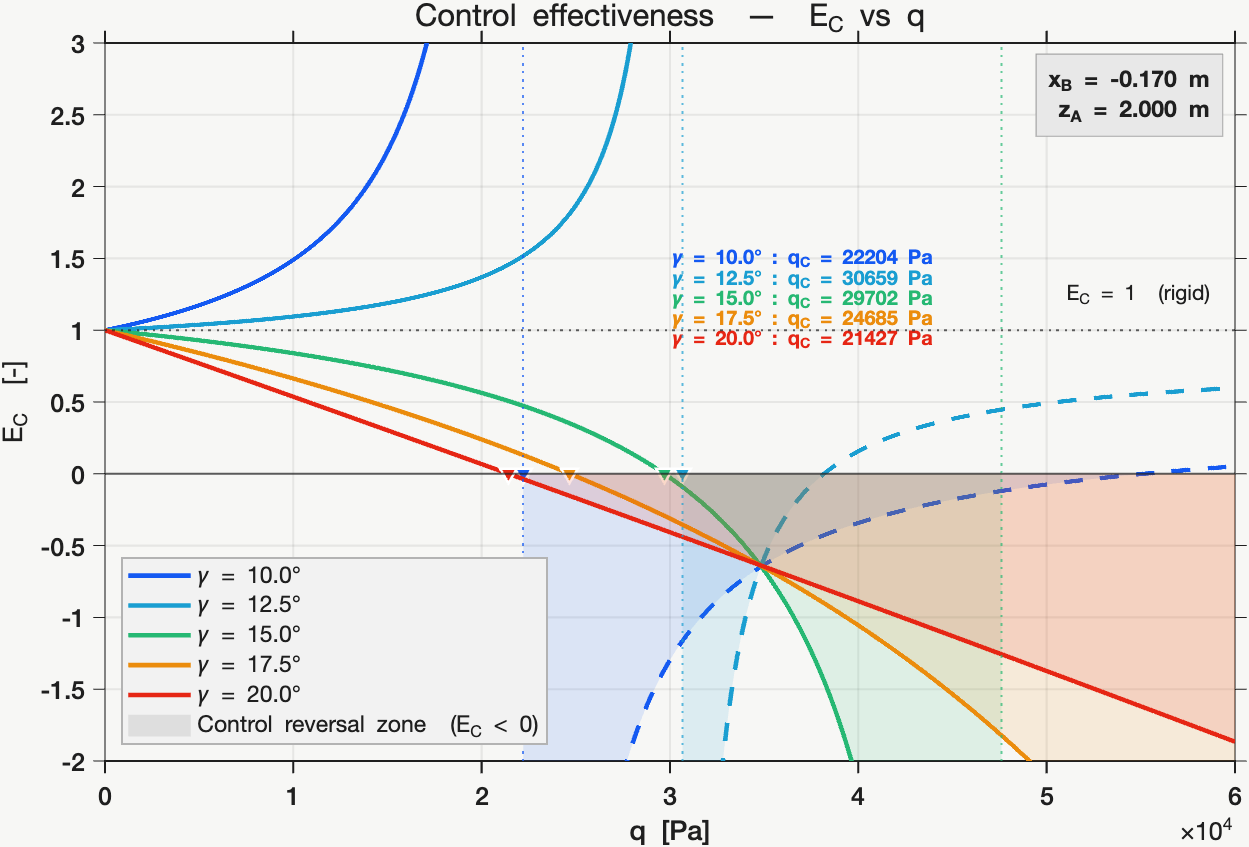
\includegraphics[width=\textwidth]{report/img/EC_vs_q_gamma.png}
\captionof{figure}{$E_C$ vs.\ $q$ for several $\gamma$, $x_B$ fixed.}
\label{fig:EC_vs_q_gamma}
\end{minipage}
\end{figure}


\section*{Comparison of the deformed shape with and without the strut}

\noindent Config: $x_B=0.10\ \mathrm{m}$, $\beta_0=10^\circ$, $q=0.4\,q_{D,0}$ (subcritical -- differences attributable to strut stiffening, not instability proximity). $\delta_z$ interpreted only for $y\ge y_{\min}=4.31\ \mathrm{m}$ ($\approx30.8\%\,b$), defined as the first station where the absolute gap at $x=c/4$ reaches $10\%$ of its tip value, to avoid the root singularity ($z_\mathrm{ns}\to0$).\\[0.5cm]
\begin{minipage}[c]{0.75\textwidth}
\centering
% Row 1
\begin{minipage}[t]{0.48\linewidth}
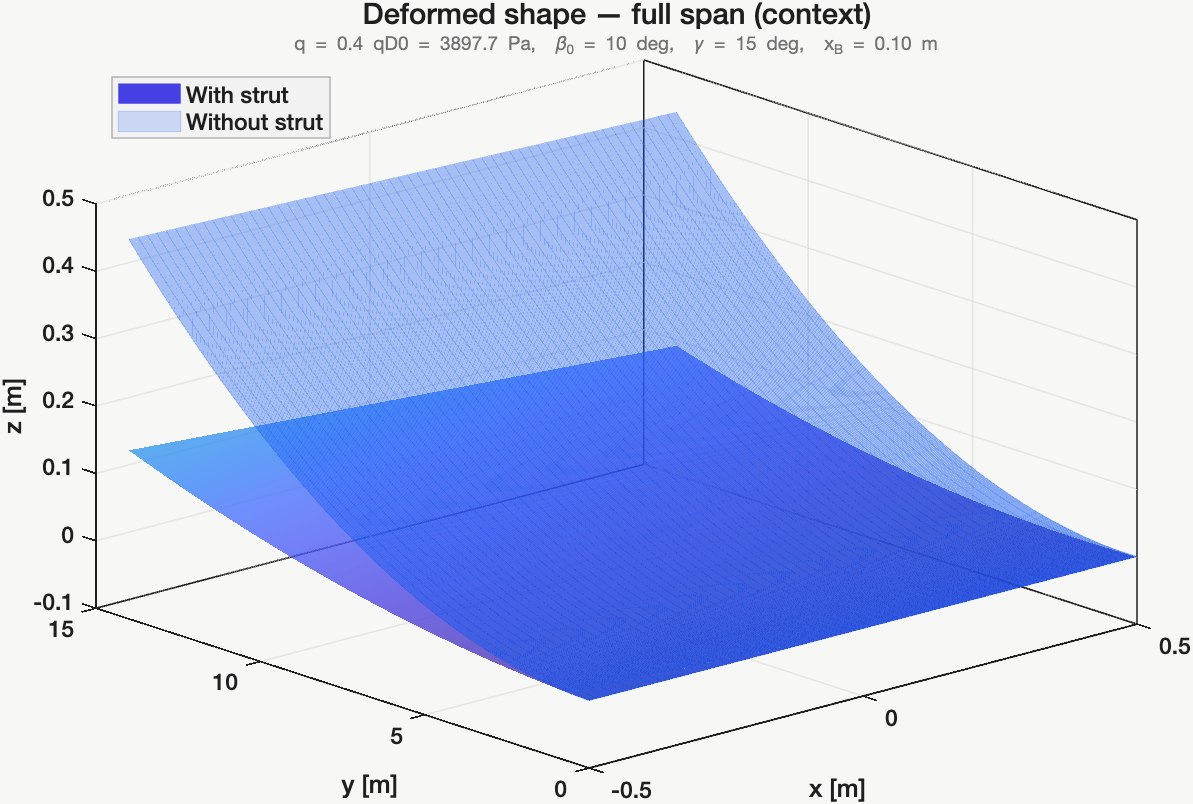
\includegraphics[width=\linewidth]{report/img/deformed_shape_fullspan.png}
\centerline{\small\textit{3D shape, with vs.\ without strut.}}
\label{fig:q3_deformed_3d}
\end{minipage}
\hfill
\begin{minipage}[t]{0.48\linewidth}
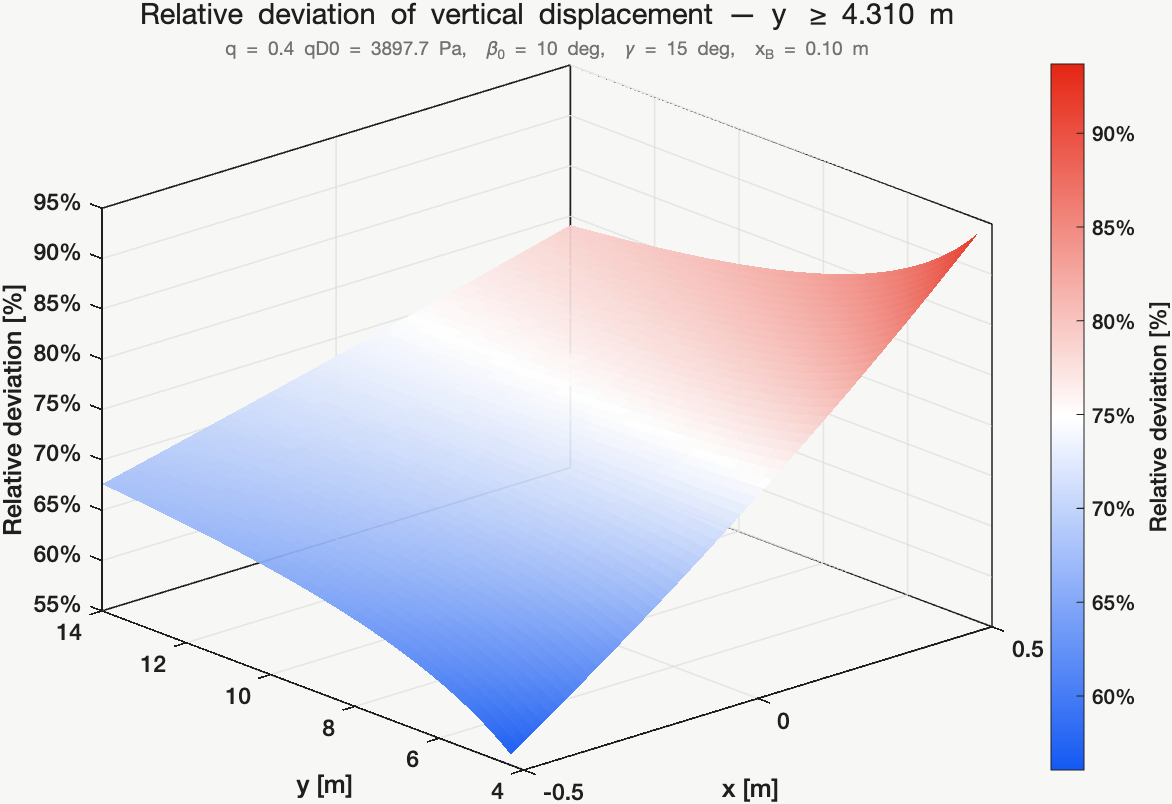
\includegraphics[width=\linewidth]{report/img/relative_deviation_3d.png}
\centerline{\small\textit{$\delta_z$ map, $y\ge y_{\min}$.}}
\label{fig:q3_rel_3d}
\end{minipage}

\vspace{0.3em}

% Row 2
\begin{minipage}[t]{0.48\linewidth}
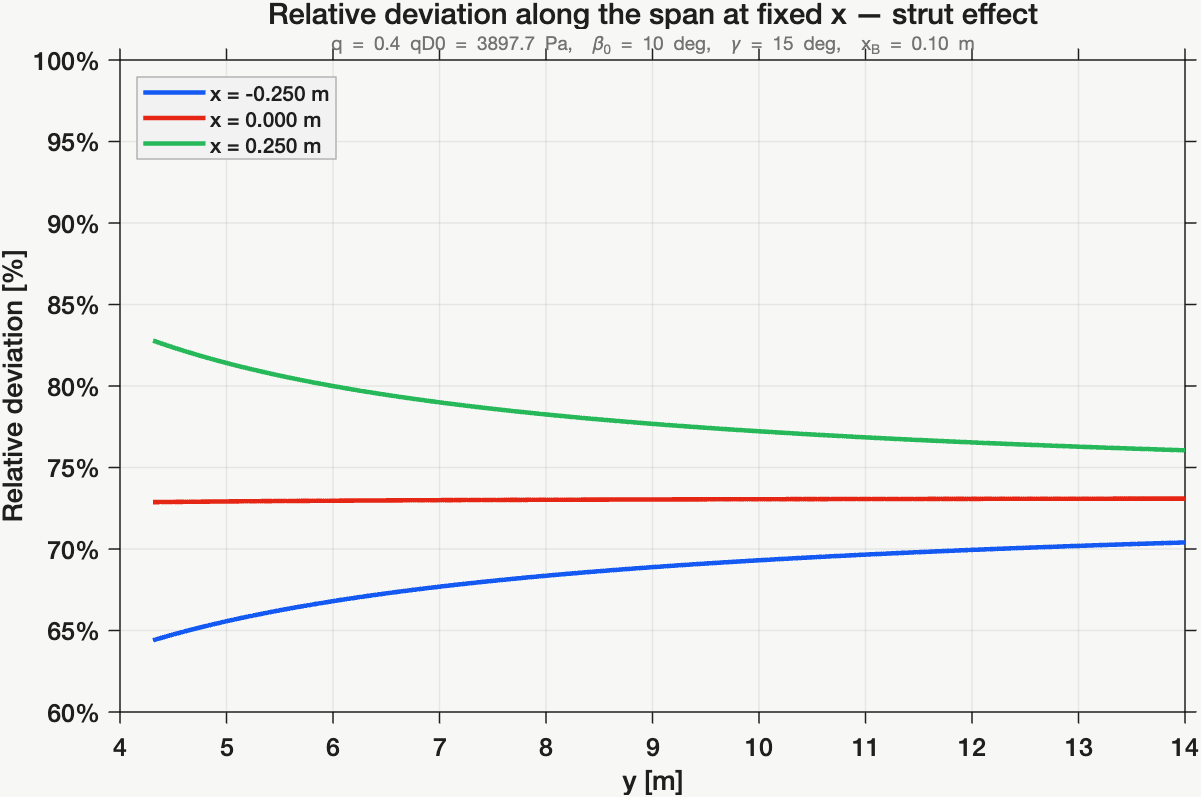
\includegraphics[width=\linewidth]{report/img/relative_deviation_spanwise.png}
\centerline{\small\textit{Spanwise cuts of $\delta_z$.}}
\label{fig:q3_rel_span}
\end{minipage}
\hfill
\begin{minipage}[t]{0.48\linewidth}
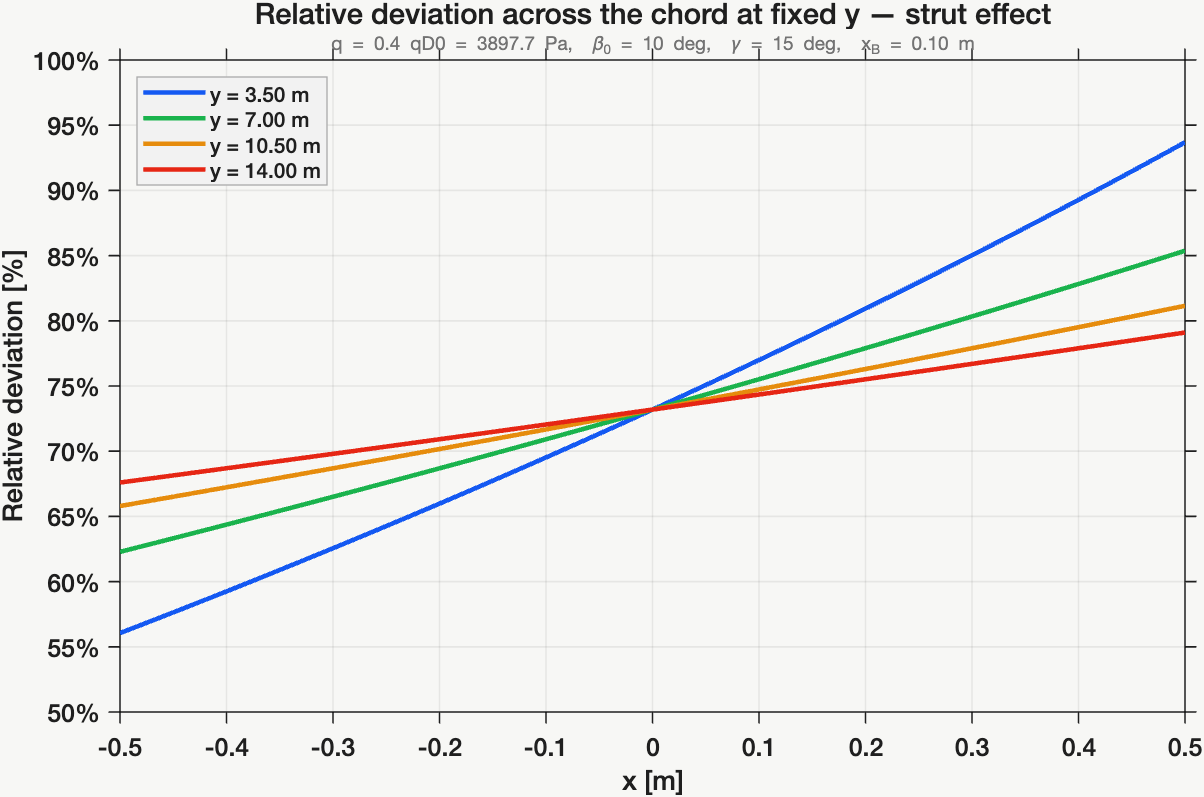
\includegraphics[width=\linewidth]{report/img/relative_deviation_chordwise.png}
\centerline{\small\textit{Chordwise cuts of $\delta_z$.}}
\label{fig:q3_rel_chord}
\end{minipage}
\end{minipage}%
\hfill%
\begin{minipage}[c]{0.22\textwidth}
\small

Both configurations share the same bending--torsion pattern (zero at root, increasing toward tip); the strut reduces amplitude without altering shape: \\

1) $\delta_z\in \sim [50\%,90\%]$ over valid span -- strut wing is $\tfrac{1}{4}$--$\tfrac{1}{3}$ as deformed as no-strut reference.\\

2) Along elastic axis ($x=0$): $z=(y/b)^2\phi_w$, $\delta_z\approx70\%$ -- dominant bending reduction.\\

3) Chordwise variation of $\delta_z$ consistent with torsional term $-x(y/b)\phi_\theta$ -- strut simultaneously stiffens bending and torsion.\\

\end{minipage}




% % ============================================================
% \section*{1. Control Effectiveness}
% % ============================================================

% The control effectiveness is defined as:

% \begin{equation}
%     \boxed{E_C(q) = 1 + q\,\frac{b}{b_a}\,\frac{C_{L\alpha}}{C_{L\beta}}
%     \cdot \frac{K_{T11}\,F_{a2} - K_{T21}\,F_{a1}}{2\,\det\mathbf{K}_\text{TOT}(q)}}
% \end{equation}

% where $\mathbf{K}_\text{TOT}(q)$ is the total stiffness matrix (structural + aerodynamic).
% The \textbf{control reversal pressure} $q_R$ is defined by:

% \begin{equation}
%     E_C(q_R) = 0, \qquad E_C(q) < 0 \;\text{ for }\; q > q_R
% \end{equation}

% % ============================================================
% \section*{2. Singularity at Divergence}
% % ============================================================

% The divergence pressure $q_D$ satisfies $\det\mathbf{K}_\text{TOT}(q_D) = 0$,
% which creates a singularity in $E_C$:

% \begin{equation}
%     E_C(q) \;\xrightarrow{q \to q_D^\pm}\; \pm\infty
% \end{equation}

% This produces a \textbf{spurious sign change} of $E_C$ at $q_D$,
% indistinguishable numerically from a physical zero crossing.
% Naive root-finding (e.g.\ \texttt{fzero} over a single interval) therefore
% fails, locking onto $q_D$ instead of $q_R$.

% Two physically distinct configurations arise depending on strut position $x_B$:

% \begin{center}
% \begin{tabular}{ccc}
% \toprule
% Case & Condition & Behaviour of $E_C$ \\
% \midrule
% $q_R < q_D$ & strut far forward & crosses $0$ from $+$ to $-$ before $q_D$ \\
% $q_R > q_D$ & strut near EA    & crosses $0$ from $-$ to $+$ after $q_D$ \\
% \bottomrule
% \end{tabular}
% \end{center}

% % ============================================================
% \section*{3. Numerical Strategy}
% % ============================================================

% The domain is split into two segments that \emph{exclude} $q_D$:

% \begin{equation}
%     \mathcal{S}_1 = \bigl[0,\; q_D - \delta\bigr], \qquad
%     \mathcal{S}_2 = \bigl[q_D + \delta,\; 50\,q_D\bigr],
%     \qquad \delta = 0.1\,q_D
% \end{equation}

% On each segment, $E_C$ is evaluated on a uniform grid of $N = 30{,}000$ points.
% Points where $|E_C| > 10^3$ are discarded (singularity filter).
% Consecutive valid points with an index gap $> 5$ are skipped (NaN cluster rejection).

% The root is accepted according to:

% \begin{itemize}
%     \item \textbf{Case 1} — $q_R < q_D$: first $+\to-$ crossing in $\mathcal{S}_1$
%     \item \textbf{Case 2} — $q_R > q_D$: first $-\to+$ crossing in $\mathcal{S}_2$,
%           provided $E_C < 0$ on the entire interval $[q_D+\delta,\; q_R]$
%           (rules out the spurious post-singularity jump)
% \end{itemize}

% Each candidate bracket is refined by \texttt{fzero} to tolerance $\varepsilon = 10^{-10}$.

